
  
\documentclass[journal,12pt,twocolumn]{IEEEtran}

\usepackage{setspace}
\usepackage{gensymb}
\singlespacing
\usepackage[cmex10]{amsmath}

\usepackage{amsthm}

\usepackage{mathrsfs}
\usepackage{txfonts}
\usepackage{stfloats}
\usepackage{bm}
\usepackage{cite}
\usepackage{cases}
\usepackage{subfig}

\usepackage{longtable}
\usepackage{multirow}

\usepackage{enumitem}
\usepackage{mathtools}
\usepackage{steinmetz}
\usepackage{tikz}
\usepackage{circuitikz}
\usepackage{verbatim}
\usepackage{tfrupee}
\usepackage[breaklinks=true]{hyperref}
\usepackage{graphicx}
\usepackage{tkz-euclide}

\usetikzlibrary{calc,math}
\usepackage{listings}
    \usepackage{color}                                            %%
    \usepackage{array}                                            %%
    \usepackage{longtable}                                        %%
    \usepackage{calc}                                             %%
    \usepackage{multirow}                                         %%
    \usepackage{hhline}                                           %%
    \usepackage{ifthen}                                           %%
    \usepackage{lscape}     
\usepackage{multicol}
\usepackage{chngcntr}

\DeclareMathOperator*{\Res}{Res}

\renewcommand\thesection{\arabic{section}}
\renewcommand\thesubsection{\thesection.\arabic{subsection}}
\renewcommand\thesubsubsection{\thesubsection.\arabic{subsubsection}}

\renewcommand\thesectiondis{\arabic{section}}
\renewcommand\thesubsectiondis{\thesectiondis.\arabic{subsection}}
\renewcommand\thesubsubsectiondis{\thesubsectiondis.\arabic{subsubsection}}


\hyphenation{op-tical net-works semi-conduc-tor}
\def\inputGnumericTable{}                                 %%

\lstset{
%language=C,
frame=single, 
breaklines=true,
columns=fullflexible
}
\begin{document}

\newcommand{\BEQA}{\begin{eqnarray}}
\newcommand{\EEQA}{\end{eqnarray}}
\newcommand{\define}{\stackrel{\triangle}{=}}
\bibliographystyle{IEEEtran}
\raggedbottom
\setlength{\parindent}{0pt}
\providecommand{\mbf}{\mathbf}
\providecommand{\pr}[1]{\ensuremath{\Pr\left(#1\right)}}
\providecommand{\qfunc}[1]{\ensuremath{Q\left(#1\right)}}
\providecommand{\sbrak}[1]{\ensuremath{{}\left[#1\right]}}
\providecommand{\lsbrak}[1]{\ensuremath{{}\left[#1\right.}}
\providecommand{\rsbrak}[1]{\ensuremath{{}\left.#1\right]}}
\providecommand{\brak}[1]{\ensuremath{\left(#1\right)}}
\providecommand{\lbrak}[1]{\ensuremath{\left(#1\right.}}
\providecommand{\rbrak}[1]{\ensuremath{\left.#1\right)}}
\providecommand{\cbrak}[1]{\ensuremath{\left\{#1\right\}}}
\providecommand{\lcbrak}[1]{\ensuremath{\left\{#1\right.}}
\providecommand{\rcbrak}[1]{\ensuremath{\left.#1\right\}}}
\theoremstyle{remark}
\newtheorem{rem}{Remark}
\newcommand{\sgn}{\mathop{\mathrm{sgn}}}
\providecommand{\abs}[1]{\vert#1\vert}
\providecommand{\res}[1]{\Res\displaylimits_{#1}} 
\providecommand{\norm}[1]{\lVert#1\rVert}
%\providecommand{\norm}[1]{\lVert#1\rVert}
\providecommand{\mtx}[1]{\mathbf{#1}}
\providecommand{\mean}[1]{E[ #1 ]}
\providecommand{\fourier}{\overset{\mathcal{F}}{ \rightleftharpoons}}
%\providecommand{\hilbert}{\overset{\mathcal{H}}{ \rightleftharpoons}}
\providecommand{\system}{\overset{\mathcal{H}}{ \longleftrightarrow}}
	%\newcommand{\solution}[2]{\textbf{Solution:}{#1}}
\newcommand{\solution}{\noindent \textbf{Solution: }}
\newcommand{\cosec}{\,\text{cosec}\,}
\providecommand{\dec}[2]{\ensuremath{\overset{#1}{\underset{#2}{\gtrless}}}}
\newcommand{\myvec}[1]{\ensuremath{\begin{pmatrix}#1\end{pmatrix}}}
\newcommand{\mydet}[1]{\ensuremath{\begin{vmatrix}#1\end{vmatrix}}}
\numberwithin{equation}{subsection}
\makeatletter
\@addtoreset{figure}{problem}
\makeatother
\let\StandardTheFigure\thefigure
\let\vec\mathbf
\renewcommand{\thefigure}{\theproblem}
\def\putbox#1#2#3{\makebox[0in][l]{\makebox[#1][l]{}\raisebox{\baselineskip}[0in][0in]{\raisebox{#2}[0in][0in]{#3}}}}
     \def\rightbox#1{\makebox[0in][r]{#1}}
     \def\centbox#1{\makebox[0in]{#1}}
     \def\topbox#1{\raisebox{-\baselineskip}[0in][0in]{#1}}
     \def\midbox#1{\raisebox{-0.5\baselineskip}[0in][0in]{#1}}
\vspace{3cm}
\title{Assignment 8}
\author{Adarsh Sai - AI20BTECH11001}
\maketitle
\newpage
\bigskip
\renewcommand{\thefigure}{\theenumi}
\renewcommand{\thetable}{\theenumi}
%Download all python codes from 
%\begin{lstlisting}
%https://github.com/Adarsh541/AI1103-prob-and-ranvar/blob/%main/Assignment8/codes/Assignment8.py
%\end{lstlisting}
%
Download latex-tikz codes from 
%
\begin{lstlisting}
https://github.com/Adarsh541/AI1103-prob-and-ranvar/blob/main/Assignment8/Assignment8.tex
\end{lstlisting}
\section{Problem(gov/stats/2015/statistics-I(1),Q.3(a))}
Let $X_1,X_2,.....,X_n$ be independent Poisson variates with $\mean{X_i}=\mu_i$.Find the conditional distribution of $X_1,...,X_n\biggr\vert\sum_{i=1}^{n}X_i=y$
\section{Solution(gov/stats/2015/statistics-I(1),Q.3(a))}
\begin{multline}
    F\cbrak{x_1,...,x_n\biggr\vert\sum_{i=1}^{n}X_i=y}=\\
    \pr{X_1\leq x_1,...,X_n\leq x_n\biggr\vert\sum_{i=1}^{n}X_i=y}
\end{multline}
\begin{align}
    =\frac{\pr{X_1\leq x_1,...,X_n\leq x_n,\sum_{i=1}^{n}X_i=y}}{\pr{\sum_{i=1}^{n}X_i=y}}
    \label{num}
\end{align}
\begin{enumerate}
\item To find numerator of $\eqref{num}$,we solve for two random variables and extend it to n random variables.
\begin{enumerate}
    \item Solving for two variables.
    Consider the sets
        \begin{align}
          \cbrak{X_1\leq x_1} \label{s1}\\
          \cbrak{X_2\leq x_2} \label{s2}\\
          \cbrak{X_1+X_2=y}\label{s3}
        \end{align}
    \begin{enumerate}
        \item If $x_1+x_2=y$.Adding $\eqref{s1}$ and $\eqref{s2}$
        \begin{align}
            X_1+X_2 \leq x_1+x_2=y \label{s4}
        \end{align}
         and the equality holds when
        \begin{align}
            X_1=x_1\\
            X_2=x_2
        \end{align}
        From $\eqref{s3}$ and $\eqref{s4}$
        \begin{align}
            X_1+X_2=y
        \end{align}
        So the intersection of the sets is
        \begin{multline}
            \cbrak{X_1\leq x_1,X_2\leq x_2,X_1+X_2=y}\\
            =\cbrak{X_1=x_1,X_2=x_2}\\
        \text{Since $X_1$ and $X_2$ are independent}\\
            \implies \pr{X_1\leq x_1,X_2\leq x_2,X_1+X_2=y}\\
            =\pr{X_1=x_1}\pr{X_2=x_2}
        \end{multline}
        \begin{align}
            &=\prod_{i=1}^2\brak{\frac{\mu_i^{x_i}e^{-\mu_i}}{x_i!}}\\
            &=\brak{e^{-\sum\mu_i}}\prod_{i=1}^2\brak{\frac{\mu_i^{x_i}}{x_i!}}
        \end{align}
        \item if $x_1+x_2<y$.Adding $\eqref{s1}$ and $\eqref{s2}$
        \begin{align}
            X_1+X_2 \leq x_1+x_2<y \label{s5}
        \end{align}
        but from $\eqref{s3}$
        \begin{align}
            X_1+X_2=y
        \end{align}
        So there exist no values for $X_1$ and $X_2$
    \end{enumerate}
    Therefore
    \begin{multline}
        \pr{X_1\leq x_1,X_2\leq x_2,X_1+X_2=y}\\=
        \begin{cases}
            0 & x_1+x_2< y\\
            \brak{e^{-\sum\mu_i}}\prod_{i=1}^2\brak{\frac{\mu_i^{x_i}}{x_i!}} & x_1+x_2=y
        \end{cases}
    \end{multline}
\end{enumerate}
Extending to n variables we get
    \begin{multline}
        \pr{X_1\leq x_1,...,X_n\leq x_n,\sum_{i=1}^{n}X_i=y}\\=
        \begin{cases}
         \brak{e^{-\sum\mu_i}}\prod_{i=1}^n\brak{\frac{\mu_i^{x_i}}{x_i!}} & \sum_{i=1}^n x_i=y\\
         0 & \sum_{i=1}^n x_i<y
        \end{cases}
        \label{n}
    \end{multline}
\item \textbf{Theorem}:If the random variables $X_1,X_2$ are independent and poisson distributed with parameters $\lambda_1,\lambda_2$,then their sum $Z=X_1+X_2$ is also poisson distributed with parameter $\lambda_1+\lambda_2$.\textbf{proof}:The characteristic function of a poisson random variable is given by
\begin{align}
    \Phi_X(\omega)=e^{-\lambda(1-e^{j\omega})}
\end{align}
Using convolution 
\begin{align}
    \Phi_Z(\omega)&=\Phi_{X_1}(\omega)\Phi_{X_2}(\omega)\\
    &=e^{-\lambda_1(1-e^{j\omega})}e^{-\lambda_2(1-e^{j\omega})}\\
    &=e^{-(\lambda_1+\lambda_2)(1-e^{j\omega})}
\end{align}
This theorem can be extended to n variables.So
\begin{align}
    \pr{\sum_{i=1}^{n}X_i=y}=\frac{\brak{\sum\mu_i}^ye^{-\sum\mu_i}}{y!}\label{den}
\end{align}
From $\eqref{num}$,$\eqref{n}$ and $\eqref{den}$ 
\begin{multline}
     F\cbrak{x_1,...,x_n\biggr\vert\sum_{i=1}^{n}X_i=y}\\=
     \begin{cases}
      \frac{y!}{\brak{\sum\mu_i}^y}\prod_{i=1}^n\brak{\frac{\mu_i^{x_i}}{x_i!}} & \sum_{i=1}^n x_i =y\\
      0 & \sum_{i=1}^n x_i<y
     \end{cases}
\end{multline}
\end{enumerate}
\begin{figure}[!ht]
\centering
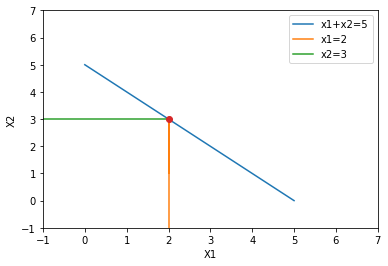
\includegraphics[width=\columnwidth]{plot1.png}
\caption{If $x_1+x_2=5$.The solution of the ordered pair $\brak{X_1,X_2}$,satisfying $\eqref{s1}$,$\eqref{s2}$ and $\eqref{s3}$, is shown by the red point(for $y=5,x_1=2,x_2=3$)  }
\end{figure}
\begin{figure}[!ht]
\centering
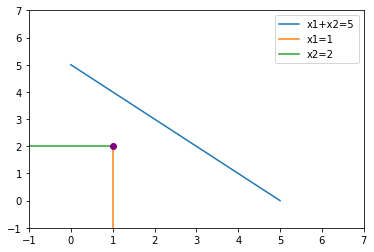
\includegraphics[width=\columnwidth]{plot2.png}
\caption{If $x_1+x_2<5$.There are no values of $\brak{X_1,X_2}$,satisfying $\eqref{s1}$,$\eqref{s2}$ and $\eqref{s3}$(for $y=5,x_1=1,x_2=2$)}
\end{figure}\begin{figure}[!ht]
\centering
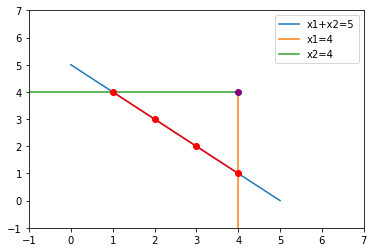
\includegraphics[width=\columnwidth]{plot3.png}
\caption{If $x_1+x_2>5$.The solution of the ordered pair $\brak{X_1,X_2}$,satisfying $\eqref{s1}$,$\eqref{s2}$ and $\eqref{s3}$, is shown by the red points(for $y=5,x_1=4,x_2=4$) }
\end{figure}
\end{document}

